%------------------------------------------------------------------------------
% Template file for the submission of papers to IUCr journals in LaTeX2e
% using the iucr document class
% Copyright 1999-2013 International Union of Crystallography
% Version 1.6 (28 March 2013)
%------------------------------------------------------------------------------

\documentclass[preprint]{iucr}              % DO NOT DELETE THIS LINE
\usepackage{amssymb}
\usepackage[fleqn]{amsmath}
%\usepackage{bm}
\usepackage{graphicx}
\usepackage{tabularx}
\usepackage{booktabs}
%\usepackage{calligra}
\usepackage{array}
\DeclareMathAlphabet{\mathcalligra}{T1}{calligra}{m}{n}
\def\mathbi#1{\textbf{\em #1}}
\numberwithin{equation}{section}
%\DeclareMathSymbol{\Gamma}{\mathalpha}{letters}{"00}
%\DeclareMathSymbol{\Lambda}{\mathalpha}{letters}{"03}
%\DeclareMathSymbol{\Omega}{\mathalpha}{letters}{"0A}
%\DeclareMathAlphabet{\mathitbf}{OML}{cmm}{b}{it}
\hyphenation{Niggli}
\def\mathbi#1{\textbf{\em #1}}
%\numberwithin{equation}{section}
%\DeclareMathSymbol{\Gamma}{\mathalpha}{letters}{"00}
%\DeclareMathSymbol{\Lambda}{\mathalpha}{letters}{"03}
%\DeclareMathSymbol{\Omega}{\mathalpha}{letters}{"0A}
%\DeclareMathAlphabet{\mathitbf}{OML}{cmm}{b}{it}
\usepackage{color}
\usepackage{ulem}
\usepackage{url}
\usepackage{yfonts}
%\usepackage{xr-hyper}
%\usepackage[draft]{hyperref}
%\usepackage{bibentry}

\usepackage{tikz}
\usetikzlibrary{arrows.meta, positioning}
\usepackage[most]{tcolorbox}


% Space macros
\usepackage{amsmath, amssymb}  % If not already included

% Crystallographic space macros
\newcommand{\HVI}{\ensuremath{\mathbf{H}^{6}}}
\newcommand{\GVI}{\ensuremath{\mathbf{G}^{6}}}
\newcommand{\SVI}{\ensuremath{\mathbf{S}^{6}}}
\newcommand{\PIII}{\ensuremath{\mathbf{P}^{3}}}
\newcommand{\FIII}{\ensuremath{\mathbf{F}^{3}}}
\newcommand{\CIII}{\ensuremath{\mathbf{C}^{3}}}
\newcommand{\RIII}{\ensuremath{\mathbb{R}^{3}}}

% a,b,c as base vectors of unit cells
\newcommand{\va}{\ensuremath{\mathbf{a}}}
\newcommand{\vb}{\ensuremath{\mathbf{b}}}
\newcommand{\vc}{\ensuremath{\mathbf{c}}}
\newcommand{\vd}{\ensuremath{\mathbf{d}}}



\newcommand{\vdotv}[2]{${{\bf #1 \cdot #2}}$}
\newcommand{\Imaginary}[0]{\mathcal{I}}
\newcommand{\Real}[0]{\mathcal{R}}
\newcommand{\Exchange}{\ensuremath{\mathcal{X}}}


\newcommand{\nounderline}[3]{\!\!\!\!\!\!\!\!\!#1,&\!\!\!\!\!\!\!\!\!#2,&\!\!\!\!\!\!\!\!\!#3}
\newcommand{\underlineab}[3]{\!\!\!\!\!\!\!\!\!\!\!\!\!\!\!\!\!\!\!\!\!\!\!\!\Exchange{}(#1),&\!\!\!\!\!\!\!\!\!\!\!\!\!\!\!\!\!\!\!\!\!\!\!\!\Exchange{}(#2),&\!\!\!\!\!\!\!\!\!#3}
\newcommand{\underlineac}[3]{\!\!\!\!\!\!\!\!\!\!\!\!\!\!\!\!\!\!\!\!\!\!\!\!\Exchange{}(#1),&\!\!\!\!\!\!\!\!\!\!\!\!\!\!\!\!\!\!\!\!\!\!\!\!#2,&\!\!\!\!\!\!\!\!\!\Exchange{}(#3)}
\newcommand{\underlinebc}[3]{\!\!\!\!\!\!\!\!\!\!\!\!\!\!\!\!\!\!\!\!\!\!\!\!#1,&\!\!\!\!\!\!\!\!\!\Exchange{}(#2),&\!\!\!\!\!\!\!\!\!\!\!\!\!\!\!\!\!\!\!\!\!\!\!\!\Exchange{}(#3)}

\newcommand{\scalar}[1]{\ensuremath{#1}}
\newcommand{\scalarsub}[2]{\ensuremath{#1_{#2}}}


\usepackage{makecell}
\renewcommand\cellalign{l}
\renewcommand\cellgape{\Gape[4pt]}


%-------------------------------------------------------------------------
% Information about journal to which submitted
%-------------------------------------------------------------------------
\journalcode{A}              % Indicate the journal to which submitted
%   A - Acta Crystallographica Section A
%   B - Acta Crystallographica Section B
%   C - Acta Crystallographica Section C
%   D - Acta Crystallographica Section D
%   E - Acta Crystallographica Section E
%   F - Acta Crystallographica Section F
%   J - Journal of Applied Crystallography
%   M - IUCrJ
%   S - Journal of Synchrotron Radiation
\makeatletter
\font\dummyft@=dummy \relax
\makeatother


\begin{document}                  % DO NOT DELETE THIS LINE
	
	%-------------------------------------------------------------------------
	% The introductory (header) part of the paper
	%-------------------------------------------------------------------------
	
	% The title of the paper. Use \shorttitle to indicate an abbreviated title
	% for use in running heads (you will need to uncomment it).
	
	% Authors' names and addresses. Use \cauthor for the main (contact) author.
	% Use \author for all other authors. Use \aff for authors' affiliations.
	% Use lower-case letters in square brackets to link authors to their
	% affiliations; if there is only one affiliation address, remove the [a].
	
	% Use \vita if required to give biographical details (for authors of
	% invited review papers only). Uncomment it.
	
	% lca IUCr id IUCr6401
	%\vita{Author's biography}
	
	% Keywords (required for Journal of Synchrotron Radiation only)
	% Use the \keyword macro for each word or phrase, e.g. 
	% \keyword{X-ray diffraction}\keyword{muscle}
	
	
	% PDB and NDB reference codes for structures referenced in the article and
	% deposited with the Protein Data Bank and Nucleic Acids Database (Acta
	% Crystallographica Section D). Repeat for each separate structure e.g
	% \PDBref[dethiobiotin synthetase]{1byi} \NDBref[d(G$_4$CGC$_4$)]{ad0002}
	
	%\PDBref[optional name]{refcode}
	%\NDBref[optional name]{refcode}
	
	%-------------------------------------------------------------------------
	% The introductory (header) part of the paper
	%-------------------------------------------------------------------------
	
	% The title of the paper. Use \shorttitle to indicate an abbreviated title
	% for use in running heads (you will need to uncomment it).
	\begin{center}
		{\LARGE \emph{\today}} \\
	\end{center}
	
	\title{\PIII, a simple metric for \HVI}
	\shorttitle{properties of \PIII}
	
	% Authors' names and addresses. Use \cauthor for the main (contact) author.
	% Use \author for all other authors. Use \aff for authors' affiliations.
	% Use lower-case letters in square brackets to link authors to their
	% affiliations; if there is only one affiliation address, remove the [a].
	
	
	\cauthor[a]{Lawrence C.}{Andrews}{larry6640995@gmail.com}{}
	\author[b]{Herbert J.}{Bernstein}
	
	\aff[a]{Ronin Institute, 9515 NE 137th St, Kirkland, WA, 98034-1820 \country{USA}}
	\aff[b]{Ronin Institute, c/o NSLS-II, Brookhaven National Laboratory, Upton, NY, 11973 \country{USA}}
	
	% Use \shortauthor to indicate an abbreviated author list for use in
	% running heads (you will need to uncomment it).
	
	\shortauthor{Andrews and Bernstein}
	
	% Use \vita if required to give biographical details (for authors of
	% invited review papers only). Uncomment it.
	
	% lca IUCr id IUCr6401
	%\vita{Author's biography}
	
	% Keywords (required for Journal of Synchrotron Radiation only)
	% Use the \keyword macro for each word or phrase, e.g. 
	% \keyword{X-ray diffraction}\keyword{muscle}
	
	\keyword{lattice}
	\keyword{unit cell}
	\keyword{polar}
	\keyword{\PIII}
	
	
	\maketitle                        % DO NOT DELETE THIS LINE
	
	\begin{synopsis}
		
	\end{synopsis}
	
	
	\newcommand{\si}{\ensuremath{s_1}}
	\newcommand{\sii}{\ensuremath{s_2}}
	\newcommand{\siii}{\ensuremath{s_3}}
	\newcommand{\siv}{\ensuremath{s_4}}
	\newcommand{\sv}{\ensuremath{s_5}}
	\newcommand{\svi}{\ensuremath{s_6}}
	
	% Scalar vectors
	\newcommand{\Svec}{\ensuremath{\{ \si, \sii, \siii, \siv, \sv, \svi \}}}
	\newcommand{\SvecA}{\ensuremath{\{ -\si, -\si+\sii, \si+\siii, \si+\sv, \si+\siv, \si+\svi \}}}
	
	% Operators / maps
	\newcommand{\OPES}{\ensuremath{E^3\!\to\!S^6}}
	\newcommand{\OPESS}{
		
		\[ E^3\!\to\!S^6 \]
		
	}
	\newcommand{\MSVI}{\ensuremath{M_{S^6}}}
	\newcommand{\MEIII}{\ensuremath{M_{E^3}}}
	
	% Symbolic markers
	\newcommand{\Plus}{\ensuremath{\mathcal{P}}}
	\newcommand{\Minus}{\ensuremath{\mathcal{M}}}
	
	
	
	\begin{abstract}
		
		
		\emph{Note:}  In his later publications, Boris Delaunay used the Russian version of his surname, Delone.
		
		
	\end{abstract}
	% Appendices appear after the main body of the text. They are prefixed by
	% a single \appendix declaration, and are then structured just like the
	% body text.
	
	
	\section{Introduction}
	
	In crystallography, cell geometry is conventionally encoded in a six-dimensional parameter space 
	\ensuremath{\HVI{}=(a,b,c, \alpha, \beta, \gamma).}\footnote{``H'' was chosen to
		honor early French crystallographer Ren\'e Just Ha\"uy.} But \HVI{} is not a metric space
	(where distances can be simply defined), and \HVI{} is not a vector space (where 
	objects can be added and subtracted). In the same sense, symmetry operations
	have no simple representations in \HVI{}. 
	
	For the above reasons, other spaces are often used to describe lattices, often for specialized purposes; see Table  \ref{tbl_spaces}. Figure \ref{fig_spaces} shows relationships between
	several of these spaces. Although some of these spaces, such as \HVI{} and	\FIII{} are in almost daily use, they are not often referred to 
	as ``spaces''. In the case of \FIII{}, symmetry elements are linear
	operations in this space, and fractional coordinates of atomic positions
	are vectors expressed in this space.
	
\begin{table}
	\label{tbl_spaces}
	\centering
	\caption{Crystallographic spaces with their scalar definitions and analytical purposes}
	\renewcommand{\arraystretch}{1.3}
	\begin{tabular}{|c|l|p{7cm}|}
		\hline
		\textbf{Space} & \textbf{Scalars / Coordinates} & \textbf{Purpose} \\

\hline
$\HVI$ &
\parbox[t]{5.5cm}{
	$a,\, b,\, c \in \mathbb{R}_{>0}$ — edge lengths\\
	$\alpha,\, \beta,\, \gamma \in (0^\circ, 180^\circ)$ — opposing angles\\
	Additionally, the sum of the angles must be less than 
	$360^\circ$ and must obey the triangle inequality
} &
Composite parameter space described as 
$\mathbb{R}_{>0}^3 \times (0^\circ, 180^\circ)^3$. 
The length dimensions are unconstrained, while the angles are 
geometrically restricted. Useful for conventional lattice 
descriptions, but limited in symmetry representation and 
metric-based classification. \\

\hline		
$\mathbf{F^3}$ &
$\vec{a},\, \vec{b},\, \vec{c} \in \mathbb{R}^3$ &
Base vector space, a frame space (or frame bundle) in \RIII. The coordinates are the 3-space 
base vectors of a unit cell. Symmetry 
operations are enumerated using this space. \\
\hline

		
		$\mathbf{P^3}$ &
		\parbox[t]{5.5cm}{
			$(|\vec{a}|,\alpha),\ (|\vec{b}|,\beta),\ (|\vec{c}|,\gamma)$\\
			$\Rightarrow$\,\\ 
			\hspace*{0.5cm}$(|\vec{a}|\cos\alpha,\, |\vec{a}|\sin\alpha$\\
		\hspace*{0.5cm}	$|\vec{b}|\cos\beta,\, |\vec{b}|\sin\beta$\\
		\hspace*{0.5cm}	$|\vec{c}|\cos\gamma,\, |\vec{c}|\sin\gamma)$ \\
		also known as: \\
		\hspace*{0.5cm}	\ensuremath{(p1,p2,p3)}. 
		} &
		Polar coordinate space defined by the map $\FIII \rightarrow \PIII$. Represents each base vector by magnitude and opposing angle, decomposed into directional components. Compact and smooth alternative to $\HVI$. \PIII{} provides a simple
		and intuitive space for representing and comparing
		 large numbers of unit cells. (This work) \\
		\hline


$\mathbf{S^6}$ &
\parbox[t]{5.5cm}{
	$s_1 = \vec{b} \cdot \vec{c},\, s_2 = \vec{a} \cdot \vec{c},\, s_3 = \vec{a} \cdot \vec{b}$\\
	$s_4 = \vec{a} \cdot \vec{d},\, s_5 = \vec{b} \cdot \vec{d},\, s_6 = \vec{c} \cdot \vec{d}$\\ \\
	\quad where $\vec{d} = -\vec{a} - \vec{b} - \vec{c}$
} &
A space used for Selling/Delone reduction. The scalars are derived from dot products between lattice vectors. Used for lattice classification described by Delaunay and for distance computation \cite{Andrews2019b}. 24 Bravais types were defined by citeasnoun{Delone1975} in \SVI{}, but 
described using pictures showing the special relationships. \citeasnoun{andrews2023measuring} revised the table of Delone to
include the \SVI vector definitions of the Bravais types.\\

		\hline
		$\mathbf{G^6}$ &
		\parbox[t]{5.5cm}{
			$g_1 = \vec{a} \cdot \vec{a},\, g_2 = \vec{b} \cdot \vec{b},\, g_3 = \vec{c} \cdot \vec{c}$\\
			$g_4 = 2\vec{b} \cdot \vec{c},\, g_5 =2 \vec{c} \cdot \vec{a},\, g_6 = 2\vec{a} \cdot \vec{b}$
		} &
		A space based on the metric tensor (and thus dot products 
		of the basis vectors of the unit cell) and used for Niggli reduction and lattice distance computation. \cite{Andrews2014}
		The International Tables for Crystallography describe the 44
		Bravais types that result from Niggli reduction using
		algebraic expression in \GVI{} (but stated in terms of scalars
		rather than manifolds in \GVI{}) \cite{ITC_VolumeA_2016}. \\
		\hline
		
\CIII &
\parbox[t]{5.5cm}{
	from the \SVI{} scalars, $s1,...,s6$\\
	$c1=(s1,s4), c2=(s2,s5), c3=(s3,s6)$\\
	where (?,?) denotes a complex number
} &
\CIII{} was created to associate related scalars after the
indication of \citeasnoun{Delone1975} concerning the ``opposite''
scalars in \SVI{}. Symmetry and Selling/Delaunay reduction have
simpler forms in \CIII{} than in \SVI{}. \cite{andrews2023complex}\\
\hline
		
		$\mathbf{DC7u}$ &
		\parbox[t]{5.5cm}{
			$d_1,\, d_2,\, d_3$ — cell edge lengths\\
			$d_4,\, d_5,\, d_6$ — shorter face diagonals' lengths\\
			$u$ — shortest body diagonal
		} &
		Unsorted Dirichlet Cell space derived from Niggli-reduced cells. Defined by the map from lattice geometry to a 7-dimensional vector of distances. Fully invertible and smooth; used for rapid lattice distance computation. \cite{bernstein2023invertible}\\
		\hline

	\end{tabular}
\end{table}

\begin{figure}
	\centering
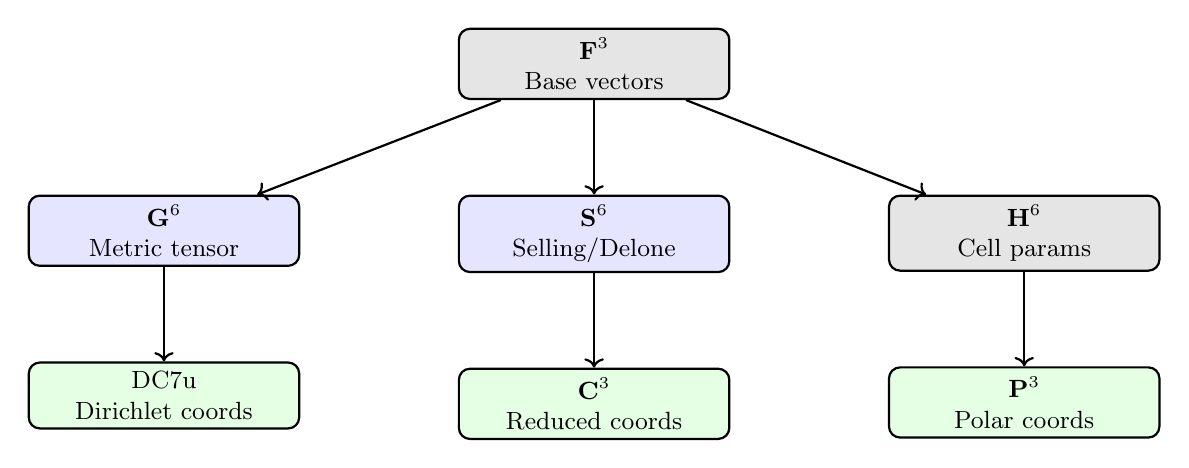
\begin{tikzpicture}[
	node distance=1.2cm and 2.0cm,
	coordspace/.style={text width=3.2cm, align=center, rectangle, draw=black,
		fill=gray!20, rounded corners, font=\small, thick},
	metricspace/.style={text width=3.2cm, align=center, rectangle, draw=black,
		fill=blue!10, rounded corners, font=\small, thick},
	derivedspace/.style={text width=3.2cm, align=center, rectangle, draw=black,
		fill=green!10, rounded corners, font=\small, thick},
	arrowlabel/.style={font=\scriptsize, midway, fill=white, inner sep=1pt}
	]
	
	% Row 1: Fundamental space
	\node[coordspace] (F3) {\FIII{} \\ Base vectors};
	
	% Row 2: Scalar & parameter spaces
	\node[metricspace] (G6) [below left=of F3] {\GVI{} \\ Metric tensor};
	\node[metricspace] (S6) [below=of F3] {\SVI{} \\ Selling/Delone};
	\node[coordspace] (H6) [below right=of F3] {\HVI \\ Cell params};
	
	% Row 3: Derived/reduced spaces
	\node[derivedspace] (DC7u) [below=of G6] {DC7u \\ Dirichlet coords};
	\node[derivedspace] (C3) [below=of S6] {\CIII{} \\ Reduced coords};
	\node[derivedspace] (P3) [below=of H6] {\PIII{} \\ Polar coords};
	
	% Arrows from F3 to row 2
	\draw[->, thick] (F3) -- (G6);
	\draw[->, thick] (F3) -- (S6);
	\draw[->, thick] (F3) -- (H6);
	
	% Arrows from row 2 to row 3
	\draw[->, thick] (G6) -- (DC7u);
	\draw[->, thick] (S6) -- (C3);
	\draw[->, thick] (H6) -- (P3);
	
\end{tikzpicture}
\label{fig_spaces}
\caption{Derived relationships among crystallographic spaces. 
	Base vector space \FIII{} gives rise to three scalar spaces:
	metric tensor space \GVI{}, Selling/Delone space \SVI{}, and conventional cell parameter space \HVI{}.
	Each transforms into a reduced or classification space: 
	$\mathbf{DC7u}$ from \GVI{}, \CIII{} from \SVI{}, and \PIII{} from $\mathbf{H^6}$.}
\end{figure}

\section{	\PIII{} Is introduced.}

\citeasnoun{Delone1975} repeatedly pointed out the relationship of the
``opposite'' scalars in the tetrahedron representations of the Selling
scalars. Examining those relationships show that the opposite terms 
are pairs where a term involving a is opposite a term involving $\alpha$, etc.

Extending the observation of \citeasnoun{Delone1975}, the idea occurs
to make a triple of variables of those pairs. Since each pair has
one length and one angle, we considered each pair as the definition of
a polar coordinate space. The result is \PIII{}, a space of 3 2-dimensional polar coordinates. See Table \ref{tbl_spaces} for the
formal description.  Two uses immediately are obvious.

The first uses the 2-dimensional character of the coordinates of \PIII{}. They
allow simple to plot representations of collections of unit cells. 
See Figure \ref{PlotPolar_raw}, Figure \ref{PlotPolar_Niggli}, and Figure \ref{PlotPolar_Delone}.

\begin{figure}
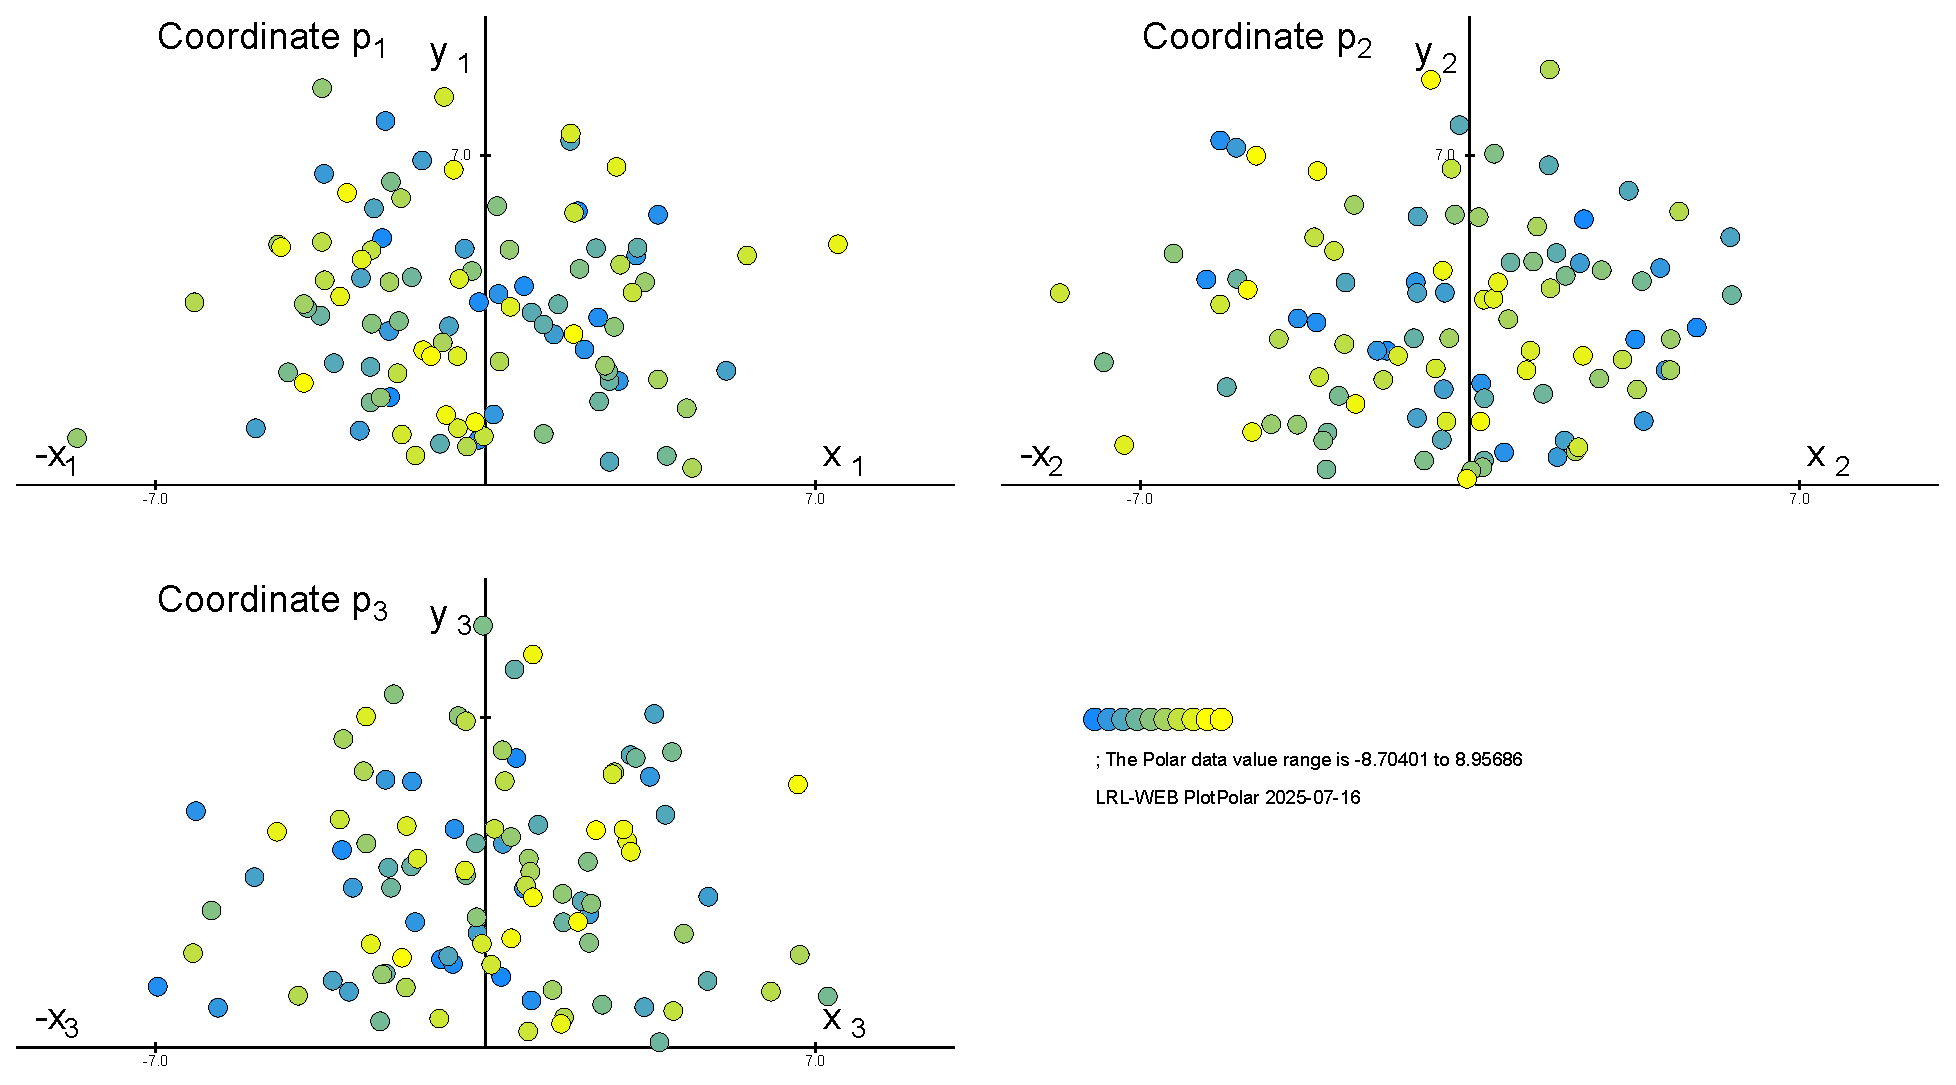
\includegraphics[width=\columnwidth]{PlotPolar_raw}
\label{PlotPolar_raw}
	\caption{100 random primitive triclinic unit cells}
\end{figure}

\begin{figure}
	\includegraphics[width=\columnwidth]{PlotPolar_Niggli}
	\label{PlotPolar_Niggli}
	\caption{The same100 random primitive triclinic unit cells, Niggli-reduced}
\end{figure}


\begin{figure}
	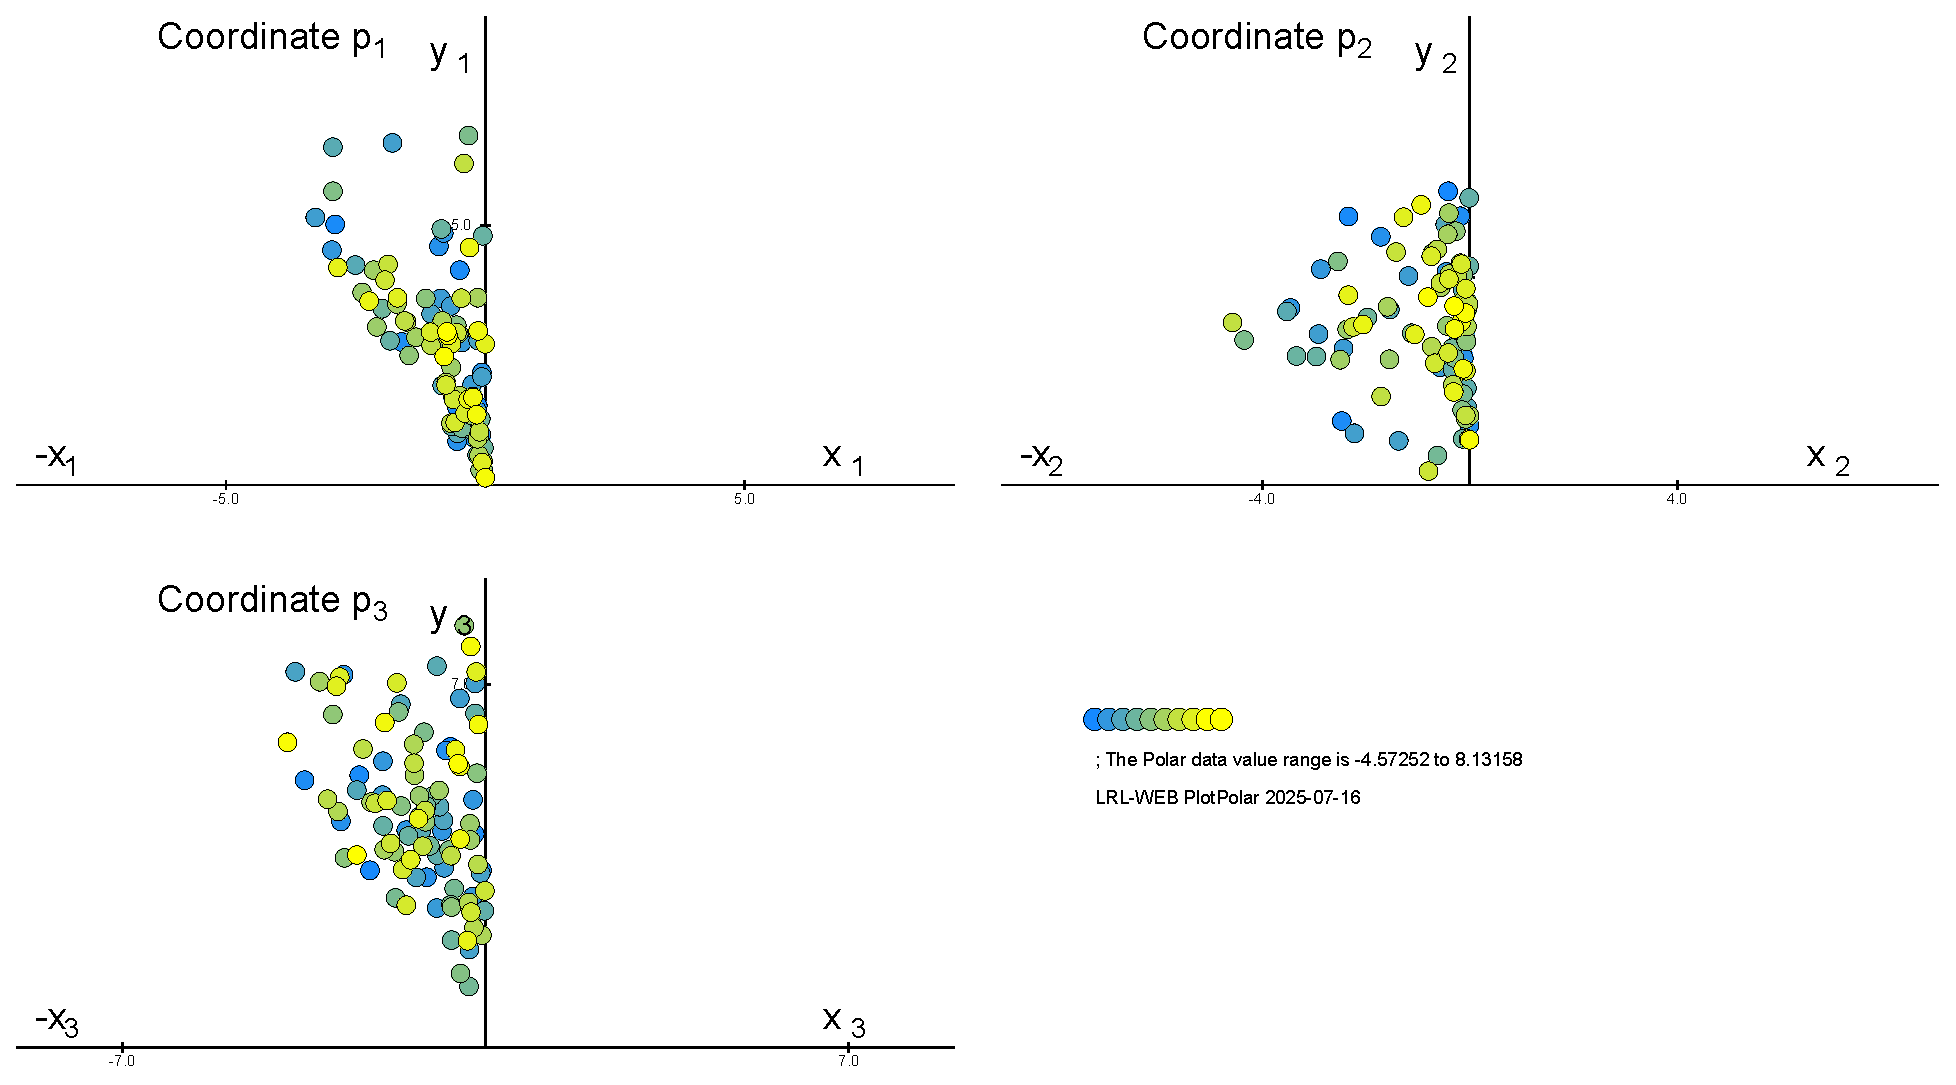
\includegraphics[width=\columnwidth]{PlotPolar_Delone}
	\label{PlotPolar_Delone}
	\caption{The same 100 random primitive triclinic unit cells, Selling-reduced}
\end{figure}

%\[
%(|\vec{x}|\cos\theta,\, |\vec{x}|\sin\theta) \in \mathbb{R}^2
%\]



%which preserves the Euclidean magnitude and implicitly encodes angular orientation. While the transformation is nonlinear in angle, the resulting structure allows straightforward computation of relative orientation, cluster proximity, and shape similarity through standard Euclidean metrics.

The second use is allowing the calculation of Euclidean distances. Because \PIII{} can be represented as 3 xy planes, the Euclidean difference between
any two unit cells described as \PIII{} can be easily computed. Thus use
contrasts with \HVI{}, where incommensurate lengths and angles do not
lend themselves to a distance calculation. 



\section{Relationship to Other Spaces}

While derived from the same foundational cell parameters as $\mathbf{H^6}$, the space $\mathbf{P^3}$ sidesteps issues of angular nonlinearity  that arise in conventional cell representations. Compared with $\mathbf{C^3}$, which seeks symmetry-reduced coordinates derived from $\mathbf{S^6}$, the construction of $\mathbf{P^3}$ is more geometric than algebraic. It provides a useful intermediary: more interpretable than metric tensors or other spaces, less abstract than \SVI{} or \GVI{}.

	
	
	\section{Notation}
	
	
	
	
	\section{Matrices of boundary transformations}
	
	
	\subsection{Derivation}
	
	
	\subsection{Example P++ implementation}
	
	
	
	
	\subsection{Example of use}
	
	
	\section{Graphical display of projections}
	
	\section{Scalar Reduction and Canonical Presentation in Projected Vector Triplets}
	
	\subsection{1. Standard Presentation of Projected Vectors}
	
	Let a set of three projected vectors be given:
	
	
	\[
	(p_1, p_2, p_3), \quad p_i \in \mathbb{R}^2
	\]
	
	
	Each \( p_i \) is constructed from a lattice vector via magnitude and opposing angle:
	
	
	\[
	p_i = |\vec{v}_i| (\cos \theta_i, \sin \theta_i)
	\]
	
	
	
	The \textbf{Standard Presentation} algorithm assigns a canonical ordering and orientation to the triplet:
	
	\begin{enumerate}
		\item \textbf{Magnitude Sort:} Reorder vectors so that
		
		
		\[
		|p_1| \leq |p_2| \leq |p_3|
		\]
		
		
		using Euclidean norms \( |p_i| = \sqrt{x_i^2 + y_i^2} \). Ties are preserved up to a numerical tolerance \( \delta \).
		
\item \textbf{Directional Coherence:} If the \( x \)-components of the triplet are not all of consistent sign, flip the necessary vectors by negating only the \( x_i \) component:


\[
p_i \to (-x_i,\ y_i)
\]


This maps quadrant I vectors into quadrant II, preserving their placement in the upper half-plane and maintaining angular conventions typical in crystallographic analysis.



\[
p_i \to (-x_i,\ y_i)
\]


to align the triplet into a directionally consistent state. If all \( x_i < 0 \), the configuration is already coherent and requires no change.

		
		
		\[
		p_i \to (-x_i, y_i)
		\]
		
		
		for any two vectors, preserving chirality.
		
		\item \textbf{Return Ordered Triplet:} Output the permuted and flipped triplet with consistent magnitude order and cosine directionality.
	\end{enumerate}
	
	\vspace{1em}
	
	\subsection{2. Scalar Projection Interaction and Cost Function}
	
	For any pair of projected vectors \( p_i, p_j \in \mathbb{R}^2 \), define the scalar projection interaction (or directional affinity):
	
	
	\[
	\mu_{ij} = p_i \cdot p_j = x_i x_j + y_i y_j
	\]
	
	
	
	The \textbf{scalar coupling cost} is then defined over the triplet as:
	
	
	\[
	C' = \frac{|\mu_{12}| + |\mu_{13}| + |\mu_{23}|}{p_1 \cdot p_1 + p_2 \cdot p_2 + p_3 \cdot p_3}
	\]
	
	
	
	This cost measures the normalized sum of pairwise directional alignment. Lower values of \( C' \) indicate that the projected vectors are less directionally coupled — i.e., more orthogonal or dispersed.
	
	\vspace{1em}
	
	\subsection{3. Scalar Reduction Algorithm}
	
	The goal of scalar reduction is to transform the triplet \( (p_1, p_2, p_3) \) into an algebraically simpler form — one with lower scalar coupling cost \( C' \) — while preserving lattice identity (e.g., volume and reconstructability).
	
	The reduction proceeds iteratively:
	
	\begin{enumerate}
		\item \textbf{Initialization:}
		Apply standard presentation. Compute initial cost \( C'_0 \) and physical volume \( V_0 > 0 \).
		
		\item \textbf{Pairwise Projection Subtractions:}
		For each unordered pair \( (p_i, p_j),\ i \neq j \), compute the scalar coefficient:
		
		
		\[
		\lambda = \frac{p_i \cdot p_j}{p_j \cdot p_j}
		\]
		
		
		Then define the candidate vector:
		
		
		\[
		p_i' = p_i - \lambda p_j
		\]
		
		
		
		\item \textbf{Evaluate Candidate:}
		Apply standard presentation to updated triplet. Recompute cost \( C'_{\text{new}} \) and volume \( V_{\text{new}} \).
		
		\item \textbf{Acceptance Criteria:}
		Accept the transformation if:
		
		
		\[
		C'_{\text{new}} + \delta < C' \quad \text{and} \quad V_{\text{new}} > 0
		\]
		
		
		
		\item \textbf{Repeat:}
		Continue until no further accepted transformations lower the cost.
		
		\item \textbf{Output:}
		Return the reduced triplet \( (p_1, p_2, p_3)_{\text{red}} \) with minimal scalar cost.
	\end{enumerate}
	
	\vspace{1em}
	
	\subsection{4. Interpretation of Cost and Reduction}
	
	The term "reduction" refers to minimizing the scalar coupling among vectors — reducing directional alignment that obscures presentation clarity. The cost \( C' \) is a rigorously defined metric for this alignment. Transformations reduce \( C' \) while preserving:
	\begin{itemize}
		\item The vector magnitudes and their reconstructable relationships
		\item The unit cell's volume and crystallographic identity
		\item The triplet’s algebraic validity in scalar projection space
	\end{itemize}
	
	Reduction leads to a cleaner, more canonical representation of the original structure — just as Niggli reduction provides a minimal cell in metric tensor space, scalar reduction provides a minimal configuration in projected vector space.
	
	
	
	
	\section{Summary}
	
	
	
	
	\section{Availability of code} CmdToP3 and PlotPolar are available in github.com, in
	\url{https://github.com/duck10/LatticeRepLib.git}.
	
	%\appendix
	
	
	%\section{blah blah blah -- Supplementary Material}
	\ack{{\bf Acknowledgements}}
	
	Careful copy-editing and corrections by Frances C. Bernstein are 
	gratefully acknowledged.
	%	Our thanks to Jean Jakoncic and Alexei Soares for 
	%	helpful conversations and access to data and facilities at 
	%	Brookhaven National Laboratory.
	%	
	\ack{{\bf Funding information}}      
	
	Funding for this research was provided in part by:  
	US Department of Energy Offices of Biological and 
	Environmental Research and of Basic Energy Sciences 
	(grant No. DE-AC02-98CH10886; grant No. E-SC0012704); 
	U.S. National Institutes of Health (grant No. P41RR012408; 
	grant No. P41GM103473; grant No. P41GM111244; 
	grant No. R01GM117126,
	grant No. 1R21GM129570); Dectris, Ltd.
	
	
	\bibliography{Reduced}
	
	\bibliographystyle{iucr}
	
	
	
	%-------------------------------------------------------------------------
	% TABLES AND FIGURES SHOULD BE INSERTED AFTER THE MAIN BODY OF THE TEXT
	%-------------------------------------------------------------------------
	
	% Simple tables should use the tabular environment according to this
	% model
	
	% Postscript figures can be included with multiple figure blocks
	
	%C:\Users\lca\Source\Repos\LatticeRepLib\x64\Debug>plotc3
	%; Graphical output SVG file =PLT__2023-03-07.13_43_35.svg
	%
	%C:\Users\lca\Source\Repos\LatticeRepLib\x64\Debug>cmdniggli | plotc3
	%; Graphical output SVG file =PLT__2023-03-07.13_44_06.svg
	%
	%C:\Users\lca\Source\Repos\LatticeRepLib\x64\Debug>cmddelone | plotc3
	%; Graphical output SVG file =PLT__2023-03-08.07_11_03.svg
	%
	%C:\Users\lca\Source\Repos\LatticeRepLib\x64\Debug>cmdniggli | cmdperturb 5 20 | plotc3
	%; Graphical output SVG file =PLT__2023-03-08.09_00_13.svg
	%
	%C:\Users\lca\Source\Repos\LatticeRepLib\x64\Debug>cmdniggli | cmdperturb 5 100 | plotc3
	%; Graphical output SVG file =PLT__2023-03-08.09_00_21.svg
	
\end{document}                    % DO NOT DELETE THIS LINE
%%%%%%%%%%%%%%%%%%%%%%%%%%%%%%%%%%%%%%%%%%%%%%%%%%%%%%%%%%%%%%%%%%%%%%%%%%%%%%
